\documentclass{beamer}
\usetheme{default}

\usepackage{graphicx}
\usepackage{multicol}
\usepackage{fancyvrb}

\newcommand{\bi}{\begin{itemize}}
\newcommand{\ii}{\item}
\newcommand{\ei}{\end{itemize}}

\newcommand{\bframe}[1]{\begin{frame}[fragile]{#1}}




\title{IF notes}
\subtitle{based on {\em The Craft of Adventure, 2nd ed.}, Graham Nelson\\
 and {\em Twisty Little Passages}, Nick Montfort}
\author{Geoffrey Matthews}


\begin{document}
\begin{frame}
\maketitle
\end{frame}
\bframe{Prehistory}
\begin{itemize}
\item Stephen Bishop
\item Explorer, Mammoth Cave, 1820-1857
\end{itemize}

\resizebox{3in}{!}{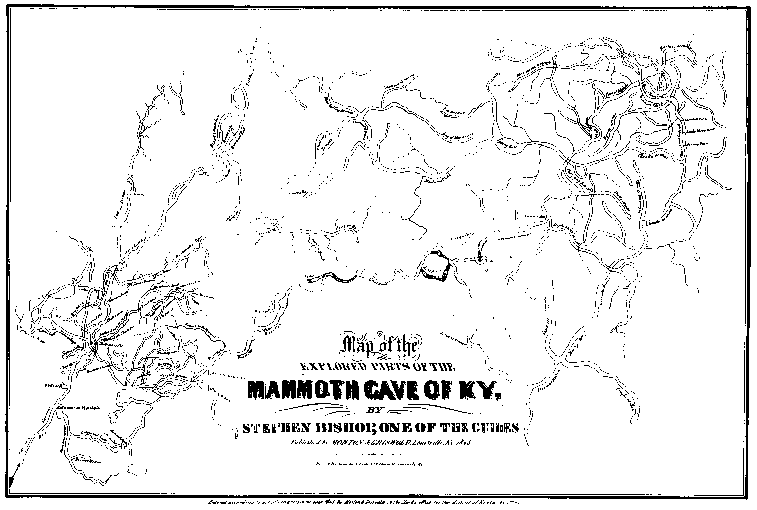
\includegraphics{MapofMammothCave.png}}

\end{frame}
\bframe{History, 1972-1981}
\begin{itemize}
\item Will Crowther
\item Explorer, Mammoth Cave
\item {\em Dungeons and Dragons} player
\item About 1972, wrote ADVENT for his children
\end{itemize}

\vspace{1cm}

{\bf At End of Road}

You are standing at the end of a road before a small brick building.
Around you is a forest.  A small stream flows out of the building
and down a gulley.

\end{frame}
\bframe{Crowther was a caver}

You are in a splendid chamber thirty feet high. The walls are frozen
rivers of orange stone. An awkward canyon and a good passage exit from
east and west sides of the chamber.

\end{frame}
\bframe{Parser Prehistory}

\begin{itemize}
\item Hunt the Wumpus
\item SHRDLU
\end{itemize}

\end{frame}
\bframe{History, 1972-1981}
\begin{itemize}
\item About 1975, Don Woods gets ahold of Crowther's ADVENT
\item Adds puzzles, pirates, vending machines {\em etc.}
\item ADVENT circulates on the ARPANET
\item {\em The Soul of a New Machine}, Tracy Kidder:  ADVENT
epitomizes the geek culture 
\item Scott Adams, many titles, simple games
\item John Laird's 'Haunt'
\item MUDs
\end{itemize}

\end{frame}

\bframe{Scott Adams}
\begin{multicols}{2}
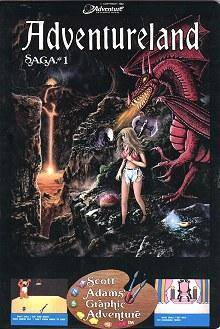
\includegraphics[width=0.5\textwidth]{Adventureland_Cover.png}
\columnbreak

Adventureland

1978

\vspace{2cm}

I'm in a dismal swamp.\\~\\

Obvious exits: North, South, East, West, Up.\\~\\

I can also see: cypress tree --- evil smelling mud --- swamp gas ---
floating patch of oily slime --- chiggers

\end{multicols}
\end{frame}

\bframe{1972-1981}

Game assemblers 

\begin{Verbatim}
JUMPHOLE:
 SKIP UNLESS R(CHAIR)R EQ HOLEROOM
 SKIP UNLESS H CHAIR PLAYER
 PRINTRET HOLEHIGH
 MOVE PLAYER WITH TO UPROOM
 PRINTRET CHAIRJUMP
\end{Verbatim}

\end{frame}
\bframe{1982-1986}

\begin{itemize}
\item MIT students built Zork
\item 1979, Started Infocom
\item Huge commercial success by 1985
\item Ran on over 20 different personal computer types
\item Business software never successful
\item Dozens of successful titles
\end{itemize}

\end{frame}
\bframe{Infocom}
\begin{multicols}{2}


\includegraphics[width=0.5\textwidth]{ZorkI.jpg}
\columnbreak

  \bi
  \item Enchanter, Sorcerer, Spellbreaker
  \item Deadline
  \item Suspended
  \item Infidel
  \item Planetfall
  \item Wishbringer
  \item Leather Goddesses of Phobos
  \item Trinity
  \ei
\end{multicols}

\end{frame}
\bframe{Sierra Online}

\resizebox{2.5in}{!}{
\includegraphics{LeisureSuitLarry.jpg}}

\end{frame}
\bframe{1982-1986}
The Golden Age
\begin{itemize}
\item {\it Amazon}, Michael Crichton
\item {\it The Hitchhiker's Guide to the Galaxy}, Douglas Adams
\item {\it Mindwheel}, Robert Pinsky (US Poet Laureate)
\item {\it I Have No Mouth and I Must Scream}, Harlan Ellison
\item {\it Gateway}, Frederik Pohl
\end{itemize}

\end{frame}
\bframe{1985-1991}
\begin{itemize}
\item Computer graphics improve
\item Market dries up
\item Infocom collapses, bought by Activision
\item Community grows  {\tt ftp.gmd.de}
\end{itemize}

\end{frame}
\bframe{1992-1999}
\begin{itemize}
\item TADS and Inform
\item Activision releases {\bf Lost Treasures of Infocom}
\item Newsgroups and the web
\item Annual contests:
\begin{itemize} 
\item GAGS (AGT) contest
\item XYZZY awards
\item SpeedIF (write a game in two hours)
\end{itemize}
\end{itemize}

\end{frame}
\bframe{Size}
Large Games:
\begin{itemize}
\item 50-60 rooms
\item 200-300 objects, 50-100 portable
\item 20,000-50,000 words
\end{itemize}

\end{frame}
\bframe{Reality}
\begin{itemize}
\item Make the game world as real as possible
\item IF should not be like a book of puzzles
\item IF should be fiction
\item ADVENT is better than Zork because its world is more authentic
(Crowther {\em vs.} Woods)
\end{itemize}

\end{frame}
\bframe{Main Characters}
\begin{itemize}
\item Triangle of Identities
\begin{itemize}
\item Player
\item Protagonist
\item Narrator
\end{itemize}
\item The parser a fourth?
\end{itemize}

\end{frame}
\bframe{\em Zork}
\begin{Verbatim}
> open the mailbox
Opening the mailbox reveals:
  A leaflet.

>ear the leaflet
I don't know the word "ear".

>eat the leaflet
Taken.
I don't think that the leaflet
   would agree with you.
\end{Verbatim}




\end{frame}
\bframe{Diegesis}
\begin{itemize}
\item Diegetic: \bi\item Drink the potion.\item Go north.\ei
\item Extradiegetic:  \bi\item Save the game.\item Restart. \ei
 \item Hypodiegetic:  \bi\item Story within a story.\ei
\item Metalepsis:  Confusing levels.
\item Example:  Music in movies.
\end{itemize}

\end{frame}
\bframe{Structure}
\begin{itemize}
\item The three act play (Hollywood movies)
\begin{itemize}
\item Act One: introductions and problems
\item Act Two: struggle and almost win
\item Act Three: final struggle
\end{itemize}
\item IF:
\begin{itemize}
\item Prologue
\item Middle Game
\item End Game
\end{itemize}
\end{itemize}

\end{frame}
\bframe{Prologue}
\begin{itemize}
\item Establish atmosphere
\item Foreshadow what is to come
\item A little background information
\item Keep the player entertained
\end{itemize}

For example: easy puzzles

\end{frame}
\bframe{Prologue to Middle Game}

\begin{itemize}
\item Transition from mundane to fantastic
\item Rewards player for playing this far
\item Promises a much richer world ahead
\end{itemize}

Example: ADVENT goes underground

\end{frame}
\bframe{Middle Game}
\begin{itemize}
\item Most structure
\item Biggest map
\item Regions or phases
\begin{itemize}
\item Parts of the map locked up until later
\item Skills the player must acquire in order to succeed
\item Items the user must attain in order to succeed
\end{itemize}
\end{itemize}

\end{frame}
\bframe{End Game}
\bi
\item Give player a sense of being near success
\item Culminate the plot
\item Reveal the game's secrets
\item Make the end match the beginning
\ei

\end{frame}
\bframe{Graphs}


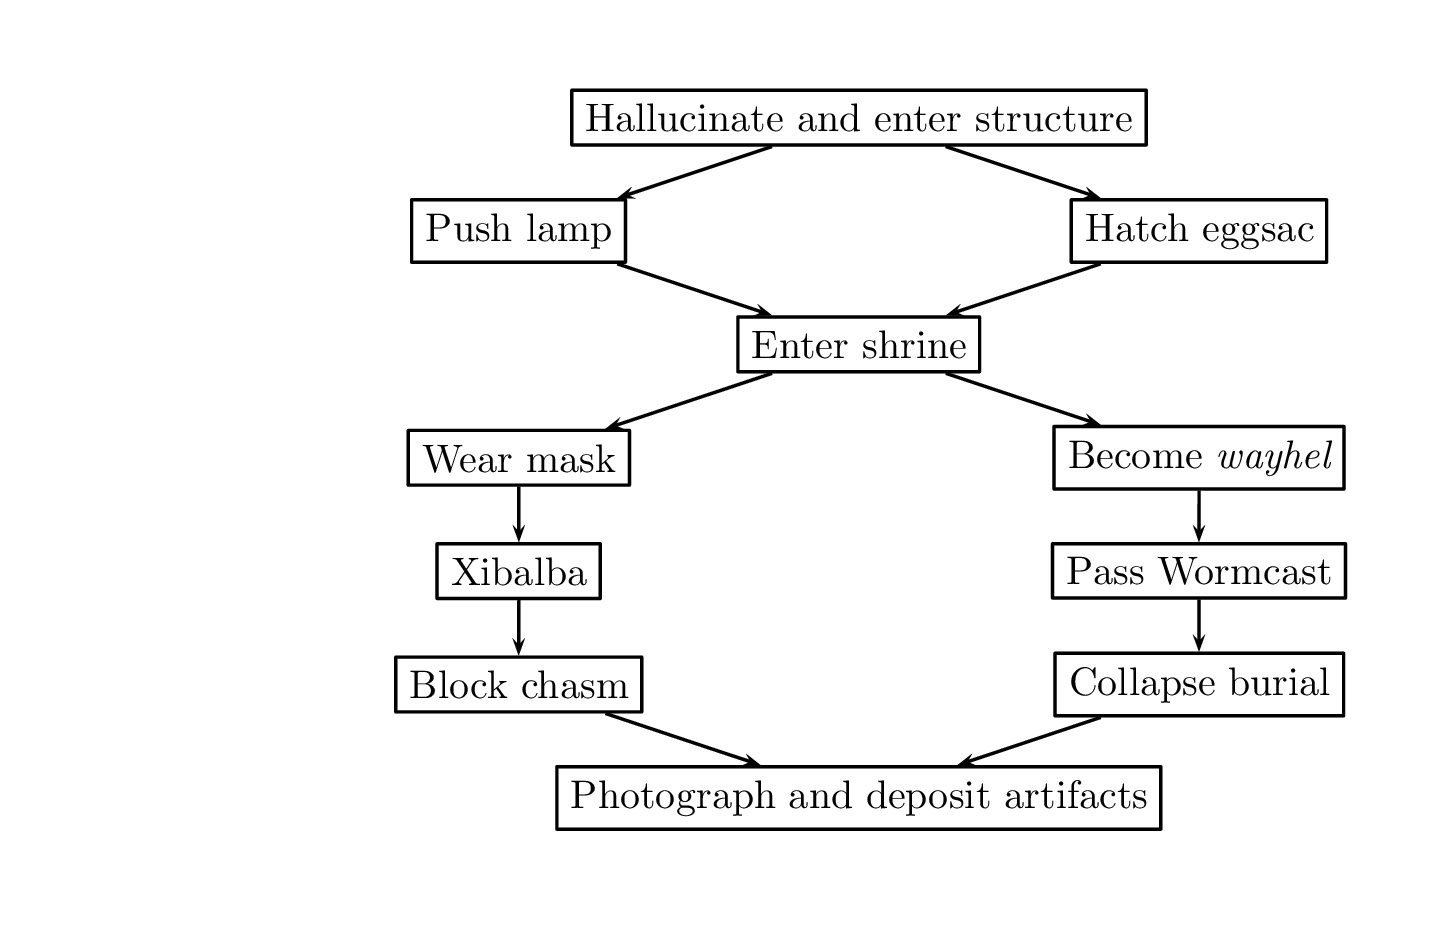
\includegraphics[width=\textwidth]{IFfigure01.png}

\end{frame}
\bframe{Graphs}
\bi
\item Is the game soluble at all?
\item How many ways?
\item How much of the game happens in different areas?
\item Is the game wide or narrow?
\item Are there bottlenecks?  They should not be too hard.
\ei

\end{frame}
\bframe{The Soul Of Drama}

{\Large
\bi
\item A character {\bf wants} something
\item An {\bf obstacle} gets in the way
\item The character takes {\bf action}
\ei
}

\vfill

If your story is lacking drama, one of these is weak.

\vfill

\end{frame}
\bframe{Bad Puzzles}
\bi
\item Too easy (single command solution)
\item Pointlessly hard (traverse the entire map to bring something
back)
\item The ``Get-X-use-X'' syndrome.  Solutions:
\bi
\item use red herrings
\item collection puzzles
\item multiple solutions
\item multiple usages
\ei
\item ``Guess the verb''
\ei

\end{frame}
\bframe{Fairness}

{\sl
Is the writer pulling a rabbit out of a hat or do
you see the fuzzy ears first?

\hfill ---Dave Lebling

\pause
\vfill

One must not put a loaded rifle on the stage if no one is thinking of firing it.

\hfill ---Anton Chekhov

\vfill
}

\end{frame}
\bframe{Puzzles}

Good approaches:
\bi
\item Write the transcript first.  Include the false tries.
\item Chain backward from a goal.  Ask yourself, ``How can I obstruct
that?''  Repeat.
\ei

\end{frame}
\bframe{Puzzle Chains}

You need to pay a debt to a Senator, so you need to steal a bust from
a temple, but that means impersonating a priest, by sacrificing a
chicken with a gladius, which means catching a chicken (you scare it
with a cat, but the cat must be attracted by a mouse, which you need
to catch with a mousetrap): and the gladius isn't just lying around,
either.  You'll need a torch, which ...

\end{frame}
\bframe{Mazes}
\bi
\item Players do {\em not} like mazes.
\item But you can be creative:
\bi
\item A new kind of map
\item A new way of seeing
\item A new kind of guide
\item New kinds of signposts
\ei
\ei

\end{frame}
\bframe{Light source puzzles}
\bi
\item Also disliked by players.
\item Finding oil, batteries, {\em etc.} gets tedious
\item Dark areas that are {\em not} meant to be lit can be creative.
\ei

\end{frame}
\bframe{Capacity puzzles}
\bi
\item Again, unpopular.
\item Limited carryall:
 Guess which three of these fifteen items you'll need next?
\item The player gets hungry, or thirsty, over and over, and must
return to the {\em same frickin' room} over and over.
\ei

\end{frame}
\bframe{Timed puzzles}
\bi
\item Once more, unpopular
\item Lead to {\em save-try-restore} loops
\item Destroy the illusion of reality
\item Events keyed to ``time of day'' can be effective.  (Everybody
knows vampires only come out at night.)
\ei

\end{frame}
\bframe{Utility objects}
\bi
\item Items that can be used again and again are popular
\item Crowbars, gloves, {\em etc.}
\ei

\end{frame}
\bframe{Locked doors}
Guarded, stuck, rusted, bolted, too heavy, ...
\bi
\item Good for pacing the game, blocking off sections of the map for a
while
\item Usually signals a new puzzle (find the key)
\item Are there people inside?  Can you knock?
\item Lockable on both sides? 
\item Does {\em locking} a door solve a puzzle?
\item Watch out for the Get-X-Use-X syndrome
\ei

\end{frame}
\bframe{Machinery and vehicles}
\bi
\item Easiest puzzles to design
\item They can have switches, handles, levers, knobs, wheels, ...
\item They don't have to say anything, but they could (signs and
labels)
\item They may require specialized tools or manuals
\item They can function as doors (chutes, dumbwaiters, conveyer belts)
\item Allow the user to learn by experimentation what the machine does
(don't call it a ``freezing machine'' or a ``wind machine'')
\ei

\end{frame}
\bframe{Some very useful puzzle items}
Because they have so many uses.
\bi
\item Fire
\item Water
\item Shovel
\item Plants
\item Animals
\item Monsters
\ei

\end{frame}
\bframe{People Puzzles}

Very difficult to program effectively

\vspace{1cm}

Example from 'Suspect':
\begin{verbatim}
>show corpse to michael
Michael doesn't appear interested.
\end{verbatim}
The body is that of Michael's wife.

\vspace{1cm}

May need to model human attitudes.  See {\em Facade} at
 \verb+http://www.interactivestory.net/+

\end{frame}
\bframe{People:  Mood maze}
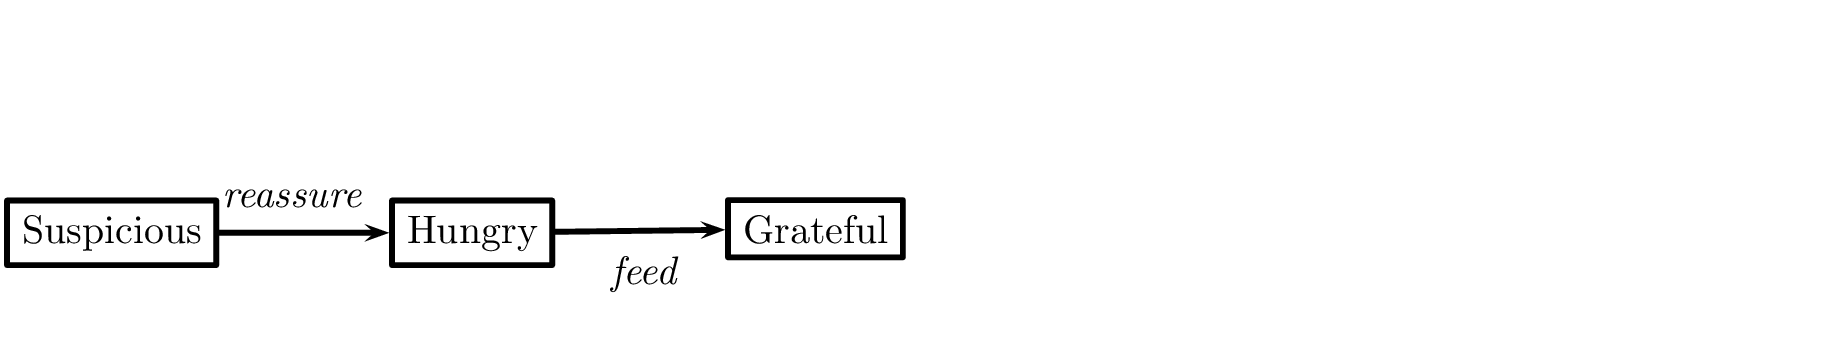
\includegraphics[scale=0.25]{IFfigure02.png}
\bi
\item Starting out in the {\em feed} direction leads nowhere
\ei

\end{frame}
\bframe{People are not automatons}
\bi
\item Should also add some spontaneous and 
random behavior to distract the player and add realism
\item See 'Galatea' for an entire game made of conversation, or
'Glass' for a short one
\ei

\end{frame}
\bframe{Dialogue Trees}
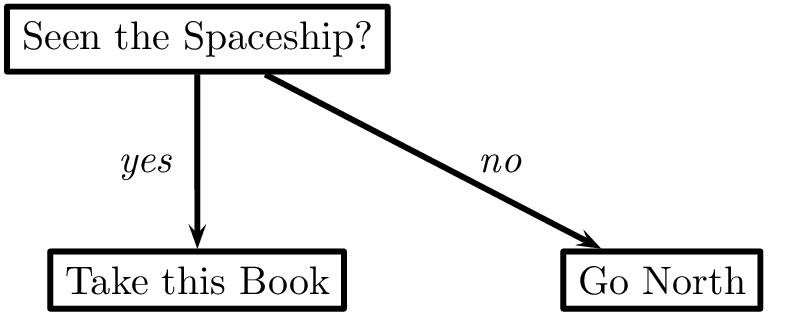
\includegraphics[scale=0.25]{IFfigure03.png}


\bi
\item Routine
\ei

\end{frame}
\bframe{Dialogue Mazes}
\bi
\item NPC can have a {\em goal} to get you to a {\em subject}.
\ei
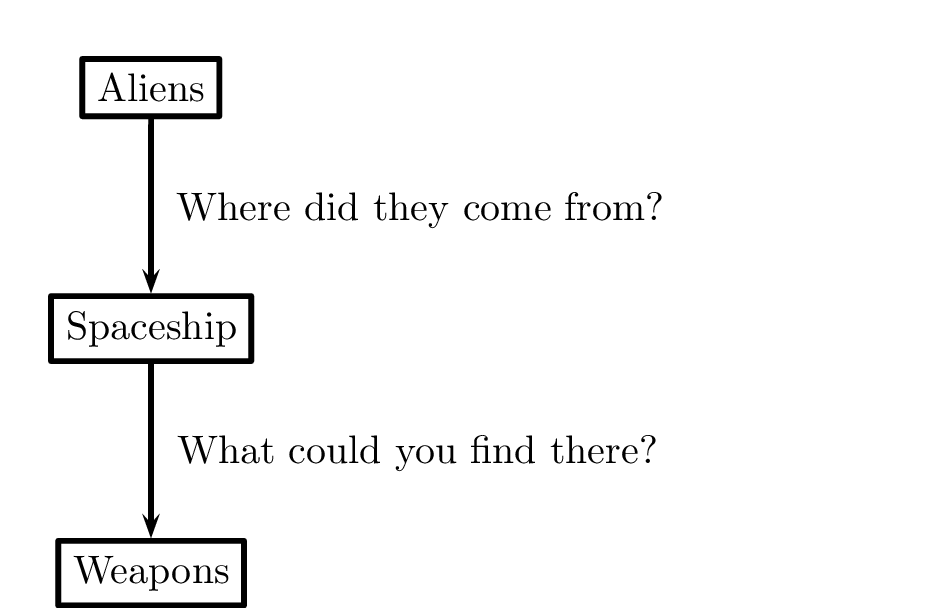
\includegraphics[scale=0.25]{IFfigure04.png}

\end{frame}
\bframe{Ropes and chains}
\bi
\item Ropes and chains are so versatile they are almost impossible to
program correctly.
\item `Otranto,' is a good example in the Inform 7 
documentation, so that a rope can be used to tie one thing to another,
climb with, and drag stuff.
\ei

\end{frame}
\bframe{Riddles}
\bi
\item Always fun
\item Symphosius:

{\small\verb+http://penelope.uchicago.edu/Thayer/E/+
\verb+      Roman/Texts/Symphosius/home.html+}

\item The Book of Exeter:

{\small
\verb+http://www.technozen.com/exeter/index.htm+
}
\ei

\end{frame}
\bframe{Symphosius}
\noindent{\it
Upon the finger my small weight is set \\
You scarce would feel my presence there, and yet \\
With my one shape, I many forms beget. \\
}

\end{frame}
\bframe{Symphosius}
\noindent{\it
Great deeds with little strength I do, \\
I close the open, ope the closed for you. \\
I keep the master's house, the master keeps me, too. \\
}

\end{frame}
\bframe{Symphosius}
\noindent{\it
The earth my body, strong through fire am I, \\
Though born of earth, my place is still on high, \\
And early drenched with dew, I soon am dry. \\
}

\end{frame}
\bframe{Book of Exeter}
\noindent{\it
I saw a creature wandering the way:\\
She was devastating---beautifully adorned.\\
On the wave a miracle:  water turned to bone.\\
}

\end{frame}
\bframe{Book of Exeter}
\noindent{\it
I'm a strange creature, for I satisfy women,\\
a service to the neighbors! No one suffers\\
at my hands except for my slayer.\\
I grow tall, erect in a bed,\\
I'm hairy underneath. From time to time\\
a good-looking girl, the doughty daughter\\
of some churl dares to hold me,\\
grips my russet skin, robs me of my head\\
and puts me in the pantry. At once that girl\\
with plaited hair who has confined me\\
remembers our meeting. Her eye moistens.\\
}

\end{frame}
\bframe{Book of Exeter}
\noindent{\it
In the town I saw a creature\\
which feeds the cattle. It has many teeth;\\
its beak is useful as it points down,\\
gently plunders and turns for home;\\
it searches for plants along the slopes,\\
and always finds those not rooted firmly;\\
it leaves the living ones held by their roots,\\
quietly standing where they spring from the soil,\\
brightly gleaming, blowing and growing.\\
}

\end{frame}
\bframe{Book of Exeter}
\noindent{\it
I'm by nature solitary, scarred by iron\\
and wounded by sword, weary of battle.\\
I often see the face of war, and fight\\
hateful enemies; yet I hold no hope\\
of help being brought to me in battle\\
before I'm cut to pieces and perish.\\
At the city wall sharp-edged sword,\\
skillfully forged in the flames by smiths,\\
bite deeply into me. I must await\\
a more fearsome encounter; it is not for me\\
to find a physician on the battlefield,\\
one of those men who heals wounds with herbs.\\
My sword wounds gape wide and wider;\\
death blows are dealt me by day and by night.\\
}


\end{frame}
\bframe{Emily Dickinson Riddles}
\begin{multicols}{2}
\noindent{\it
I like to see it lap the miles,\\
And lick the valleys up,\\
And stop to feed itself at tanks;\\
And then, prodigious, step\\
~\\
Around a pile of mountains,\\
And, supercilious, peer\\
In shanties by the sides of roads;\\
And then a quarry pare\\
}
\columnbreak
\noindent{\it
To fit its sides, and crawl between,\\
Complaining all the while\\
In horrid, hooting stanza;\\
Then chase itself down hill\\
~\\
And neigh like Boanerges; \\
Then, punctual as a star, \\
Stop---docile and omnipotent---\\
At its own stable door.\\
}
\end{multicols}



\end{frame}
\bframe{Emily Dickinson Riddles} 
\begin{multicols}{2}
\noindent{\it\small
It sifts from Leaden Sieves ---~\\
It powders all the Wood.~\\
It fills with Alabaster Wool~\\
The Wrinkles of the Road ---~\\
~\\
It makes an Even Face~\\
Of Mountain, and of Plain ---~\\
Unbroken Forehead from the East~\\
Unto the East again ---~\\
~\\
It reaches to the Fence ---~\\
It wraps it Rail by Rail~\\
Till it is lost in Fleeces ---~\\
It deals Celestial Vail~\\
}
\columnbreak
\noindent{\it\small
To Stump, and Stack---and Stem---~\\
A Summer's empty Room---~\\
Acres of Joints, where Harvests were,~\\
Recordless, but for them---~\\
~\\
It Ruffles Wrists of Posts~\\
As Ankles of a Queen---~\\
Then stills its Artisans---like Ghosts---~\\
Denying they have been---~\\
}
\end{multicols}

\end{frame}
\bframe{Emily Dickinson Riddles} 
\begin{multicols}{2}
\noindent{\it\small
A narrow fellow in the grass~\\
Occasionally rides;~\\
You may have met him,--did you not,\\
His notice sudden is.~\\
~\\
The grass divides as with a comb,~\\
A spotted shaft is seen;~\\
And then it closes at your feet~\\
And opens further on.~\\
~\\
He likes a boggy acre,~\\
A floor too cool for corn.~\\
Yet when a child, and barefoot,~\\
I more than once, at morn,~\\
}
\columnbreak
\noindent{\it\small
Have passed, I thought, a whip-lash~\\
Unbraiding in the sun,--~\\
When, stooping to secure it,~\\
It wrinkled, and was gone.~\\
~\\
Several of nature's people~\\
I know, and they know me;~\\
I feel for them a transport~\\
Of cordiality;~\\
~\\
But never met this fellow,~\\
Attended or alone,~\\
Without a tighter breathing,~\\
And zero at the bone.~\\
}
\end{multicols}

\end{frame}
\bframe{Decipherment}
\bi
\item Secret codes, if they are more than simple ciphers, are usually
enjoyed.
\item Rebus, picture language, {\em etc.} should fit with the
character of the game (hieroglyphics for pyramids)
\ei

\end{frame}
\bframe{Puzzles:  Clues}
\bi
\item Hints should be provided in-game for the difficult puzzles.
\item In modern IF, clues are essential and you should, with {\em
very} careful reading, be able to solve puzzles on the first go.
\item Can be literal (muddy footprints) or literary (puns, genre, {\em
etc.})
\item Generally, eschew in-jokes. Although in this context, references
to WWU or the Comp Sci Department faculty are probably OK.
\ei

\end{frame}
\bframe{Luck}
\bi
\item Small chance variations add fun
\item The pirate in ADVENT, the thief in Zork
\item Can be overdone
\item Can lead to the Save-Try-Restore cycle
\ei

\end{frame}
\bframe{Multiple solutions}
\bi
\item Good puzzles have many solutions, adding to the realism
\item There are seven ways to open the child-proof medicine bottle in
'Curses'. 
\item 'Wishbringer' has a magic stone to solve puzzles, but can only
be used seven times.  
\bi
\item The user of the magic stone can choose which puzzles are too
hard, this time around.
\ei
\ei

\end{frame}
\bframe{Puzzle Rewards}
\bi
\item The player gets to continue the game.
\item But there should also be an immediate reward, more items, more
rooms, more information, ...
\ei

\end{frame}
\bframe{Room Descriptions}
\bi
\item Write them properly as you go.
\item Important for the story.
\item Nothing more depressing than having nothing left but 50 rooms to
describe.  Prose suffers.
\item Describe the room sparingly, and let the object descriptions
carry some of the work.
\item Don't be flippant.
\item Use subtle humor:  {\em On the wall by the bed is a slightly
curved, full-length mirror.  You reflect upon this for a while.}
\ei

\end{frame}
\bframe{Exits}
\bi
\item Describe exits better than: ``You can go up, down, or north.''
\item Sometimes you don't have to describe exits:

{\tt
>south\\
The only exit is back out north to the sea-shore.
}
\ei

\end{frame}
\bframe{Eschew ``you''}
\bi
\item You are in ...
\item You find yourself in ...
\item This is ...
\item You have come to ...
\ei

Just describe the room:\\~\\
{\bf Fort James}\\ The enclosure of Fort James is a large, roughly
hexagonal court walled with heavy stone.  The walls face the entrance
to Port Royal Harbour, and the battery of guns is prepared to destroy
any enemy ship arriving.

\vspace{1cm}


\end{frame}
\bframe{Vocabulary Counts}

 Be specific:
\bi
\item A tree ...
\pause\\ An aged elm ...
\pause\item A car ...
\pause \\ A silver Ferrari F430 Spider ...
\pause\item A man ...
\pause\\ A wretched soul, pulling scraps of food from the dumpster,
gray wisps of hair floating from beneath a greasy stocking cap, ...
\ei


\end{frame}
\bframe{Eschew adjectives}

{\em Whirlpool Room}

You are in a magnificent cavern with a rushing stream, which cascades
over a sparkling waterfall into a roaring whirlpool which disappears
through a hole in the floor.

\end{frame}
\bframe{Write using all senses}

{\em Whirlpool Ledge}

\vspace{1cm}

The path runs a quarter-circle from south to west around a broken
ledge of this funnel cavern.  A waterfall drops out of the darkness,
catching the lamplight as it cascades into the basin.  Rapid currents
whip into a roaring whirlpool below.

\vspace{1cm}

Blue-green algae hangs in clusters from the old guard-railing, which
has almost rusted clean through in the frigid, soaking air.

\end{frame}
\bframe{Good writing is suggestive}

\bi
\item Is there a use for iron oxide from the rust?
\item Are there insect-eggs in the algae, usable for bait?
\item Can you break off the railing itself and use pieces of it?
\item Can you dive into the pool below?
\item Is there something dry which would become wet if I brought it
here?
\item Does the water have a hypnotic effect when you stare at it?
\ei

\end{frame}
\bframe{Multiple descriptions}
\bi
\item Different times of day can affect the description
\item Different lights can reveal things (ultraviolet lamps)
\item Different characters can see the room differently (dogs
sniffing)
\item 'Suspended' sees things through several different robots.
\ei

\end{frame}
\bframe{Scoring}
\bi
\item Award ranks as player accumulates score
\item Probably no ``perfect'' score, since there are many paths
through these games.
\item Some games have no score at all, but ``right'' and ``wrong''
endings. 
\ei

\end{frame}
\bframe{Testing}
\bi
\item Gareth Rees kept a log of all 475 modifications to
'Christminster'
\bi
\item 224 reports requested additional interactivity
\item 86 incorrect responses of inconsistencies
\item 32 typographical errors
\item 79 mistakes in computer programming
\ei
\ei

\end{frame}
\bframe{Handling All Input}

Most of the player's time at the keyboard is spent trying incorrect
things, and so the game is judged by how well it deals with those.

\vspace{1cm}
{\tt
In the aquarium is a baby sea-serpent who eyes you suspiciously.  His
scaly body writhes about in the huge tank.\\~\\
>\pause Take serpent\\~\\
\pause He takes you instead.  *Uurrp!*
}

\end{frame}
\bframe{Bugs}

From 'Suspect':
\vspace{1cm}

{\tt
>bartender, give me a drink\\
\pause "Sorry, I've been hired to mix drinks and that's all."
\\
~\\
\pause
>dance with alicia\\
\pause Which Alicia do you mean, Alicia or the overcoat?
\\
~\\
\pause
>talk to veronica\\
\pause Veronica's body is listening.
}

\end{frame}
\end{document}
